\documentclass[11pt]{article}
% Shared preamble for the notes in this repository. pdfLaTeX, TeX Live 2024 or later.
\usepackage[a4paper,margin=2.6cm]{geometry}
\usepackage[T1]{fontenc}
\usepackage{lmodern}
\usepackage{microtype}
\usepackage{amsmath,amssymb,amsthm}
\usepackage{graphicx}
\usepackage{booktabs}
\usepackage{enumitem}
\usepackage[dvipsnames]{xcolor}
\usepackage[hidelinks]{hyperref}
\hypersetup{colorlinks=true,linkcolor=MidnightBlue,citecolor=MidnightBlue,urlcolor=MidnightBlue}
\graphicspath{{../../figures/}}
\setlist{itemsep=2pt,topsep=4pt}

\newtheorem{theorem}{Theorem}
\newtheorem{proposition}[theorem]{Proposition}
\newtheorem{corollary}[theorem]{Corollary}
\newtheorem{conjecture}[theorem]{Conjecture}
\theoremstyle{definition}
\newtheorem{definition}[theorem]{Definition}
% Reusable derivations, numbered note.k; each note sets \notenumber. Indexed in DERIVATIONS.md.
\newcommand{\notenumber}{0}
\newtheorem{derivation}{Derivation}
\renewcommand{\thederivation}{\notenumber.\arabic{derivation}}
\newtheorem{question}{Question}
\theoremstyle{remark}
\newtheorem{remark}[theorem]{Remark}

\newcommand{\Z}{\mathbb{Z}}
\newcommand{\Q}{\mathbb{Q}}
\newcommand{\R}{\mathbb{R}}
\newcommand{\C}{\mathbb{C}}
\newcommand{\HH}{\mathbb{H}}
\newcommand{\SL}{\mathrm{SL}}
\newcommand{\Gal}{\mathrm{Gal}}
\newcommand{\Hom}{\mathrm{Hom}}
\newcommand{\repo}{\href{https://github.com/rmorleysmith/l-functions-and-physics}{\texttt{l-functions-and-physics}}}
\newcommand{\formal}{\href{https://github.com/rmorleysmith/morley-smith-formal}{\texttt{morley-smith-formal}}}
\newcommand{\script}[1]{\href{https://github.com/rmorleysmith/l-functions-and-physics/blob/main/scripts/#1}{\texttt{scripts/#1}}}
% A path inside the Lean repository; it may break after a slash.
\newcommand{\leanpath}[1]{\nolinkurl{#1}}

% Grades used in every status table.
\newcommand{\gradeLean}{\textsc{lean}}      % proved in Lean 4 with Mathlib
\newcommand{\gradeClassical}{\textsc{classical}}  % a published theorem, cited
\newcommand{\gradeComputed}{\textsc{computed}}    % checked numerically by a script in this repository
\newcommand{\gradeConvention}{\textsc{convention}}  % a choice of units or names
\newcommand{\gradeOpen}{\textsc{open}}      % a question, conjecture or working hypothesis
% The legend printed under every status table.
\newcommand{\gradelegend}{\par\nopagebreak\smallskip\noindent\begin{minipage}{\textwidth}\small
\gradeLean: proved in Lean 4 with Mathlib.
\gradeClassical: a published theorem.
\gradeComputed: checked numerically by a script in the repository \repo.
\gradeConvention: a choice of units or names.
\gradeOpen: a question, conjecture or working hypothesis.
\end{minipage}\par\medskip}
% A plain-language physical reading, placed after each derivation.
\newcommand{\physical}{\paragraph{In physical terms.}}

\renewcommand{\notenumber}{11}

\title{Three laws for a lattice of impulses}
\author{Richard Morley-Smith}
\date{Note 11 \quad November 2026}

\begin{document}
\maketitle

\begin{abstract}
\noindent
We collect the results of notes 01 to 10 into three equations for one physical system: a cubic lattice of unit impulses, observed from one of its sites.
The first says that the echoes and the tones of the lattice are the same list of integers.
The second says that the strength of an echo is a Dirichlet $L$-value at the edge of the critical strip.
The third says that the squared shape of the shell that sends the echo is an $L$-value at the centre of the strip.
Each law is stated in one line, read in physical terms, and graded.
The second, the headline law $E_N = L(1,\chi_D)/\zeta(2)$, is a theorem in every part. The second is then read as a statement about powder diffraction, and the laws are written as one set, followed by a record, in order of time, of whose theorems they are.
\end{abstract}

\section{The system}

Place a unit impulse at every point of $\Z^3$ and let it propagate by the wave equation with speed $c = 1$ (note~10).
An observer at the origin receives the $N$-th shell of neighbours, the $r_3(N)$ lattice points at distance $\sqrt N$, at the time $\sqrt N$.
Write $D$ for the discriminant of $\Q(\sqrt{-N})$, $\chi_D$ for its quadratic character, and $a(N)$ for the hexadecapole of the shell, the first coefficient of its shape (note~10, Derivation~10.3).

\section{The headline law}

Of the three laws below, one is a theorem in every part and can be stated in a line.
For a cubic lattice of unit flashes, the $N$-th echo heard at a lattice site has strength
\[
  \boxed{\;E_N = \frac{L(1,\chi_D)}{\zeta(2)}\;}\qquad(N\ \text{squarefree},\ N\not\equiv7\pmod 8),
\]
where $E_N = r_3(N)/(4\pi\sqrt N)$ is the coefficient of the wave equation's response and $\chi_D$ is the quadratic character of $\Q(\sqrt{-N})$.
The left side is a measurement on a wave; the right side is a value of a Dirichlet $L$-function.
It is Gauss's theorem on three squares combined with Dirichlet's class number formula and Kirchhoff's solution of the wave equation.

\section{Where the law is measured}

The law of size is a statement about a laboratory measurement.
A powder of a crystal with a primitive cubic lattice of side $a$ diffracts X-rays of wavelength $\lambda$ into rings, one for each shell of the reciprocal lattice: the ring of index $N = h^2+k^2+l^2$ lies at the Bragg angle $\sin\theta_N = (\lambda/2a)\sqrt N$, and its intensity carries the multiplicity factor $m_N = r_3(N)$, the number of reflections $(h,k,l)$ that fall on it~\cite{Cullity}.
For squarefree $N\not\equiv 7\pmod 8$ the law of size therefore reads
\[
  \boxed{\;m_N = \frac{24}{\pi}\,\sqrt N\,L(1,\chi_D)\;}
\]
and the law of silence says that the rings $N = 7, 15, 23, 28, 31, 39,\dots$ are absent from every primitive cubic pattern.

\physical
The multiplicity of a ring on a powder photograph is a Dirichlet $L$-value: $m_1 = 6$ is $L(1,\chi_{-4}) = \pi/4$, Leibniz's series.
The gap after the sixth line of a primitive cubic pattern, which crystallographers use to tell it from a body-centred one, is Legendre's theorem on three squares.

\section{The three laws}

\begin{derivation}[the law of duality]\label{d:duality}
For $t>0$,
\[
  \sum_{N\ge1}\frac{r_3(N)}{4\pi\sqrt N}\,\delta(t-\sqrt N) \;=\; t+\sum_{N\ge1}r_3(N)\,\frac{\sin(2\pi\sqrt N\,t)}{2\pi\sqrt N}.
\]
\end{derivation}

\physical
What arrives in time (left) equals what resonates in frequency (right), and both are weighted by the same integers.
This is Poisson summation in three dimensions; in the trace formula of note~09 the two sides are the primes and the zeros of $\zeta$.

\begin{derivation}[the law of size]\label{d:size}
For squarefree $N\not\equiv7\pmod8$,
\[
  \boxed{\;\frac{r_3(N)}{4\pi\sqrt N} = \frac{L(1,\chi_D)}{\zeta(2)}\;}
\]
and $r_3(N) = 0$ exactly when $N = 4^a(8b+7)$.
\end{derivation}

\physical
The loudness of the $N$-th echo is the value of an $L$-function at $s=1$, measured against $\zeta(2)$.
The echoes numbered $7, 15, 23, 28,\dots$ do not exist (Figure~\ref{fig:laws}).

\begin{derivation}[the law of shape]\label{d:shape}
For squarefree $N\not\equiv7\pmod8$, with $F$ the newform of weight 10 and level 2,
\[
  \boxed{\;\frac{a(N)^2}{N^{9/2}} = \frac{L(5,F\otimes\chi_D)}{L(5,F\otimes\chi_{-4})}\;}
\]
\end{derivation}

\physical
The energy in the shape of the $N$-th shell, relative to the first shell, is the value of an $L$-function at the centre of its critical strip.
Together the two boxed laws give the roundness of a shell,
$\mu_3(N)^2 = \dfrac{\pi^2}{100}\,\dfrac{L(5,F\otimes\chi_D)}{L(5,F\otimes\chi_{-4})\,L(1,\chi_D)^2\sqrt N}$:
size at the edge of the strip, shape at its centre, and a factor $1/\sqrt N$ that is the roundness of random points.

\begin{figure}[ht]
  \centering
  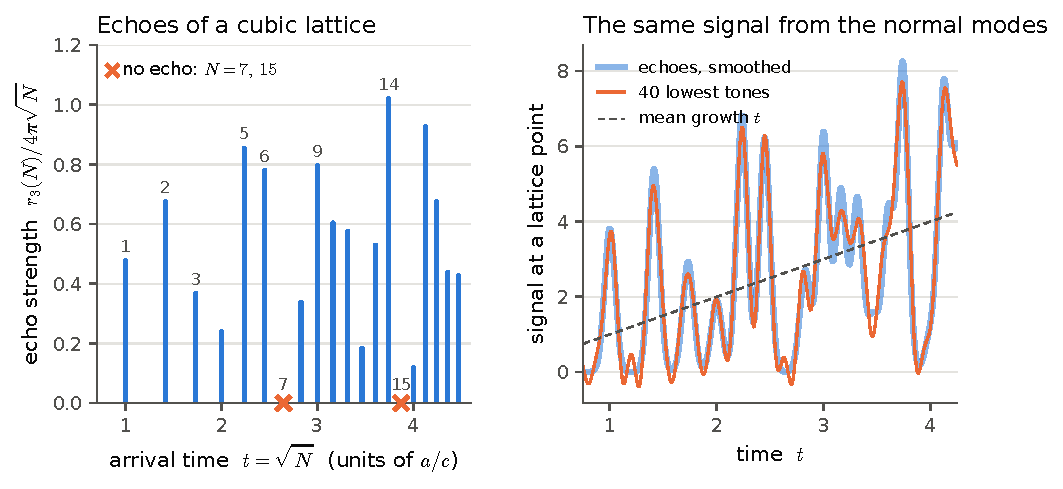
\includegraphics[width=0.94\textwidth]{spheres-echoes}
  \caption{The laws of size and duality. Left: the echo strengths $L(1,\chi_D)/\zeta(2)$, with the missing echoes. Right: the same signal from the normal modes.}
  \label{fig:laws}
\end{figure}

\section{The laws together}

Written as one set, in the manner of Maxwell's equations, with $E_N = r_3(N)/(4\pi\sqrt N)$ the strength of the $N$-th echo and $S_N = a(N)^2/N^{9/2}$ the energy in its shape:
\[
\boxed{\;
\begin{aligned}
  \textstyle\sum_{N\ge1} E_N\,\delta(t-\sqrt N) &= t+\textstyle\sum_{N\ge1} r_3(N)\,\frac{\sin(2\pi\sqrt N\,t)}{2\pi\sqrt N} &&\text{(duality)}\\[2pt]
  E_N\,\zeta(2) &= L(1,\chi_D) &&\text{(size)}\\[2pt]
  S_N\,L(5,F\otimes\chi_{-4}) &= L(5,F\otimes\chi_D) &&\text{(shape)}\\[2pt]
  E_N = 0 &\iff N = 4^a(8b+7) &&\text{(silence)}
\end{aligned}\;}
\]
The first and last lines hold for every $N$; the second and third for squarefree $N\not\equiv7\pmod 8$.

\physical
Maxwell's equations tie a field to its sources. These four lines tie a wave to arithmetic: on the left of each is something an observer at a lattice site can measure with a clock and a detector, on the right an invariant of the field $\Q(\sqrt{-N})$.
By Dirichlet's formula the second line also reads, for $N>3$, $r_3(N) = 12\,h(D)$ when $N\equiv1,2\pmod4$ and $24\,h(D)$ when $N\equiv3\pmod8$ (note~08): the echo counts the classes of binary quadratic forms of discriminant $D$.

\section{Whose theorems these are}

Every line above was found by someone else. In order of time:

\begin{description}\setlength{\itemsep}{1pt}
\item[Huygens, 1690.] Each point of a wavefront is a source of the next front~\cite{Huygens}. In three dimensions the fronts are sharp, which is why the echoes are separate clicks.
\item[Legendre, 1798, and Gauss, 1801.] Legendre stated which integers are sums of three squares; Gauss proved it and counted the representations by classes of binary quadratic forms~\cite{Gauss,Grosswald}. This is the law of silence and half of the law of size.
\item[Poisson, 1820s.] The summation formula that exchanges a lattice with its dual~\cite{SteinWeiss}. This is the law of duality.
\item[Jacobi, 1829.] The theta function and its transformation law~\cite{Jacobi}, the generating function of every shell count in these notes.
\item[Dirichlet, 1839.] The class number formula: the number of classes of forms is a value $L(1,\chi)$~\cite{Dirichlet}. This is the other half of the law of size.
\item[Riemann, 1859.] The duality of the theta function continues $\zeta$ to the whole plane and gives its functional equation; the primes are then governed by its zeros~\cite{Edwards}.
\item[Dedekind, 1877.] The eta function~\cite{Dedekind}, from which the forms $\psi$ and $F$ of the law of shape are built, and whose transformation law carries the twelve tones of note~01.
\item[Kirchhoff, 1883.] The solution of the wave equation in three dimensions by spherical means~\cite{Kirchhoff}; it turns the count $r_3(N)$ into the strength $E_N$.
\item[Klein, 1884.] The invariant forms of the finite rotation groups~\cite{Klein} (note~10, Derivation~10.6).
\item[Ewald, 1921.] Lattice sums in crystals computed by dividing the work between the lattice and its dual~\cite{Ewald}: the law of duality as a working method of physics.
\item[Bragg, 1913, and Debye and Scherrer, 1916.] Diffraction by a crystal and by a powder: each shell of the reciprocal lattice is one ring, weighted by its number of points~\cite{Cullity}.
\item[Hecke, from 1920.] $L$-functions attached to characters of number fields~\cite{Hecke} and, later, the operators and $L$-functions of modular forms.
\item[Shimura, 1973.] The correspondence between forms of half-integral weight and forms of even integral weight~\cite{Shimura}; it takes the hexadecapole series of note~10 to $F$.
\item[Montgomery, 1973, with Dyson.] The pair correlation of the zeros of $\zeta$, recognised by Dyson as that of the eigenvalues of random Hermitian matrices~\cite{Montgomery,Dyson} (note~09).
\item[Deligne, 1974.] The bound on the coefficients of cusp forms~\cite{Deligne}: shells in four dimensions are as round as chance allows.
\item[Waldspurger, 1981.] Squares of coefficients of forms of half-integral weight are central values of twisted $L$-functions~\cite{Waldspurger}. This is the law of shape.
\item[Iwaniec, 1987, and Duke, 1988.] The bound for half-integral weight and the equidistribution of lattice points on spheres in three dimensions~\cite{Iwaniec87,Duke}.
\item[Berry and Keating, 1999.] The zeros of $\zeta$ read as energy levels of a quantum system whose classical periodic orbits are the primes~\cite{BerryKeating} (note~09).
\end{description}

\noindent
Our contribution is the arrangement: one physical system in which each of these theorems is a measurable statement.

\section*{Status of the statements}

\begin{center}
\small
\begin{tabular}{@{}p{0.64\textwidth}l@{}}
\toprule
Statement & Grade\\
\midrule
Derivation~\ref{d:duality}; checked with Gaussian smoothing to $10^{-13}$ & \gradeClassical, \gradeComputed\\
Derivation~\ref{d:size}; checked for 151 values of $N\le300$ and $N\le3000$ & \gradeClassical, \gradeComputed\\
Derivation~\ref{d:shape}: proportionality within each class of $N$ in $\Q_2^\times$ modulo squares & \gradeClassical\\
Derivation~\ref{d:shape}: one constant for all seven classes, the 201 values of $N\le400$, to $10^{-11}$ & \gradeComputed\\
The formula for $\mu_3(N)^2$ & \gradeComputed\\
Powder rings: $m_N = r_3(N)$, Bragg's law (physics) & \gradeClassical\\
$m_N = (24/\pi)\sqrt N\,L(1,\chi_D)$, 151 values of $N\le300$ & \gradeClassical, \gradeComputed\\
Silence: no echo at $N = 4^a(8b+7)$ (\leanpath{MorleySmithFormal/SilentShells} in \formal) & \gradeLean\\
Silence: an echo at every other $N$ (Legendre, Gauss) & \gradeClassical\\
\bottomrule
\end{tabular}
\end{center}
\gradelegend

\noindent
All checks are in \script{spheres.py} and \script{shape\_law.py}; further references are in note~10.

\begin{thebibliography}{99}\small
\bibitem{BerryKeating} M.~V. Berry and J.~P. Keating, The Riemann zeros and eigenvalue asymptotics, \emph{SIAM Rev.} 41 (1999), 236--266.
\bibitem{Cullity} B.~D. Cullity, \emph{Elements of X-Ray Diffraction}, Addison-Wesley, 1956.
\bibitem{Dedekind} R.~Dedekind, Schreiben an Herrn Borchardt \"uber die Theorie der elliptischen Modul-Functionen, \emph{J. reine angew. Math.} 83 (1877), 265--292.
\bibitem{Deligne} P.~Deligne, La conjecture de Weil. I, \emph{Publ. Math. Inst. Hautes \'Etudes Sci.} 43 (1974), 273--307.
\bibitem{Dirichlet} P.~G. Lejeune Dirichlet, Recherches sur diverses applications de l'analyse infinit\'esimale \`a la th\'eorie des nombres, \emph{J. reine angew. Math.} 19 (1839), 324--369; 21 (1840), 1--12.
\bibitem{Duke} W.~Duke, Hyperbolic distribution problems and half-integral weight Maass forms, \emph{Invent. Math.} 92 (1988), 73--90.
\bibitem{Dyson} F.~Dyson, Birds and frogs, \emph{Notices Amer. Math. Soc.} 56 (2009), 212--223.
\bibitem{Edwards} H.~M. Edwards, \emph{Riemann's Zeta Function}, Academic Press, 1974 (with a translation of Riemann's paper of 1859).
\bibitem{Ewald} P.~P. Ewald, Die Berechnung optischer und elektrostatischer Gitterpotentiale, \emph{Ann. Phys.} 369 (1921), 253--287.
\bibitem{Gauss} C.~F. Gauss, \emph{Disquisitiones Arithmeticae}, Leipzig, 1801.
\bibitem{Grosswald} E.~Grosswald, \emph{Representations of Integers as Sums of Squares}, Springer, 1985.
\bibitem{Hecke} E.~Hecke, Eine neue Art von Zetafunktionen und ihre Beziehungen zur Verteilung der Primzahlen. Zweite Mitteilung, \emph{Math. Z.} 6 (1920), 11--51.
\bibitem{Huygens} C.~Huygens, \emph{Trait\'e de la lumi\`ere}, Leiden, 1690.
\bibitem{Iwaniec87} H.~Iwaniec, Fourier coefficients of modular forms of half-integral weight, \emph{Invent. Math.} 87 (1987), 385--401.
\bibitem{Jacobi} C.~G.~J. Jacobi, \emph{Fundamenta nova theoriae functionum ellipticarum}, K\"onigsberg, 1829.
\bibitem{Kirchhoff} G.~Kirchhoff, Zur Theorie der Lichtstrahlen, \emph{Ann. Phys.} 254 (1883), 663--695.
\bibitem{Klein} F.~Klein, \emph{Vorlesungen \"uber das Ikosaeder}, Teubner, 1884.
\bibitem{Montgomery} H.~L. Montgomery, The pair correlation of zeros of the zeta function, in \emph{Analytic Number Theory}, Proc. Sympos. Pure Math. 24, American Mathematical Society, 1973, 181--193.
\bibitem{Shimura} G.~Shimura, On modular forms of half integral weight, \emph{Ann. of Math.} 97 (1973), 440--481.
\bibitem{SteinWeiss} E.~M. Stein and G.~Weiss, \emph{Introduction to Fourier Analysis on Euclidean Spaces}, Princeton University Press, 1971.
\bibitem{Waldspurger} J.-L. Waldspurger, Sur les coefficients de Fourier des formes modulaires de poids demi-entier, \emph{J. Math. Pures Appl.} 60 (1981), 375--484.
\end{thebibliography}

\end{document}
